\chapter{Support Vector Machine (SVM)}

Support vector machine is another simple algorithm that every machine learning expert should have in his/her arsenal. Support vector machine is highly preferred by many as it produces significant accuracy with less computation power. Support Vector Machine, abbreviated as SVM can be used for both regression and classification tasks. But, it is widely used in classification objectives.\\

If we look at the cost function of logistic regression, what we'll find is that each example (x,y) contributes a term to the overall cost function.\\

\begin{center}
	$$J(\theta) = -\frac{1}{m}\sum_{i=1}^{m}\left[y^{(i)}\cdot log(h_\theta(x^{(i)})) +(1-y^{(i)})\cdot log(1-h_\theta(x^{(i)}))\right] $$
\end{center}

When y is equal to one we get the left term: 

\begin{center}
\Large{
$- y \cdot log \frac{1}{1 + e^{ - \theta^T x}} $}
\end{center}

And if we plot this function as a function of z, what we find is that we get this curve shown on the lower left of the next figure. And thus, we also see that when z is equal to large, that is, when theta transpose x is large, that corresponds to a value of z that gives us a fairly small value, a very small contribution to the consumption. And this kinda explains why, when logistic regression sees a positive example, with y=1, it tries to set theta transport x to be very large because that corresponds to this term, in the cross function, being small. \\

\begin{figure}[h!]
	\centering
	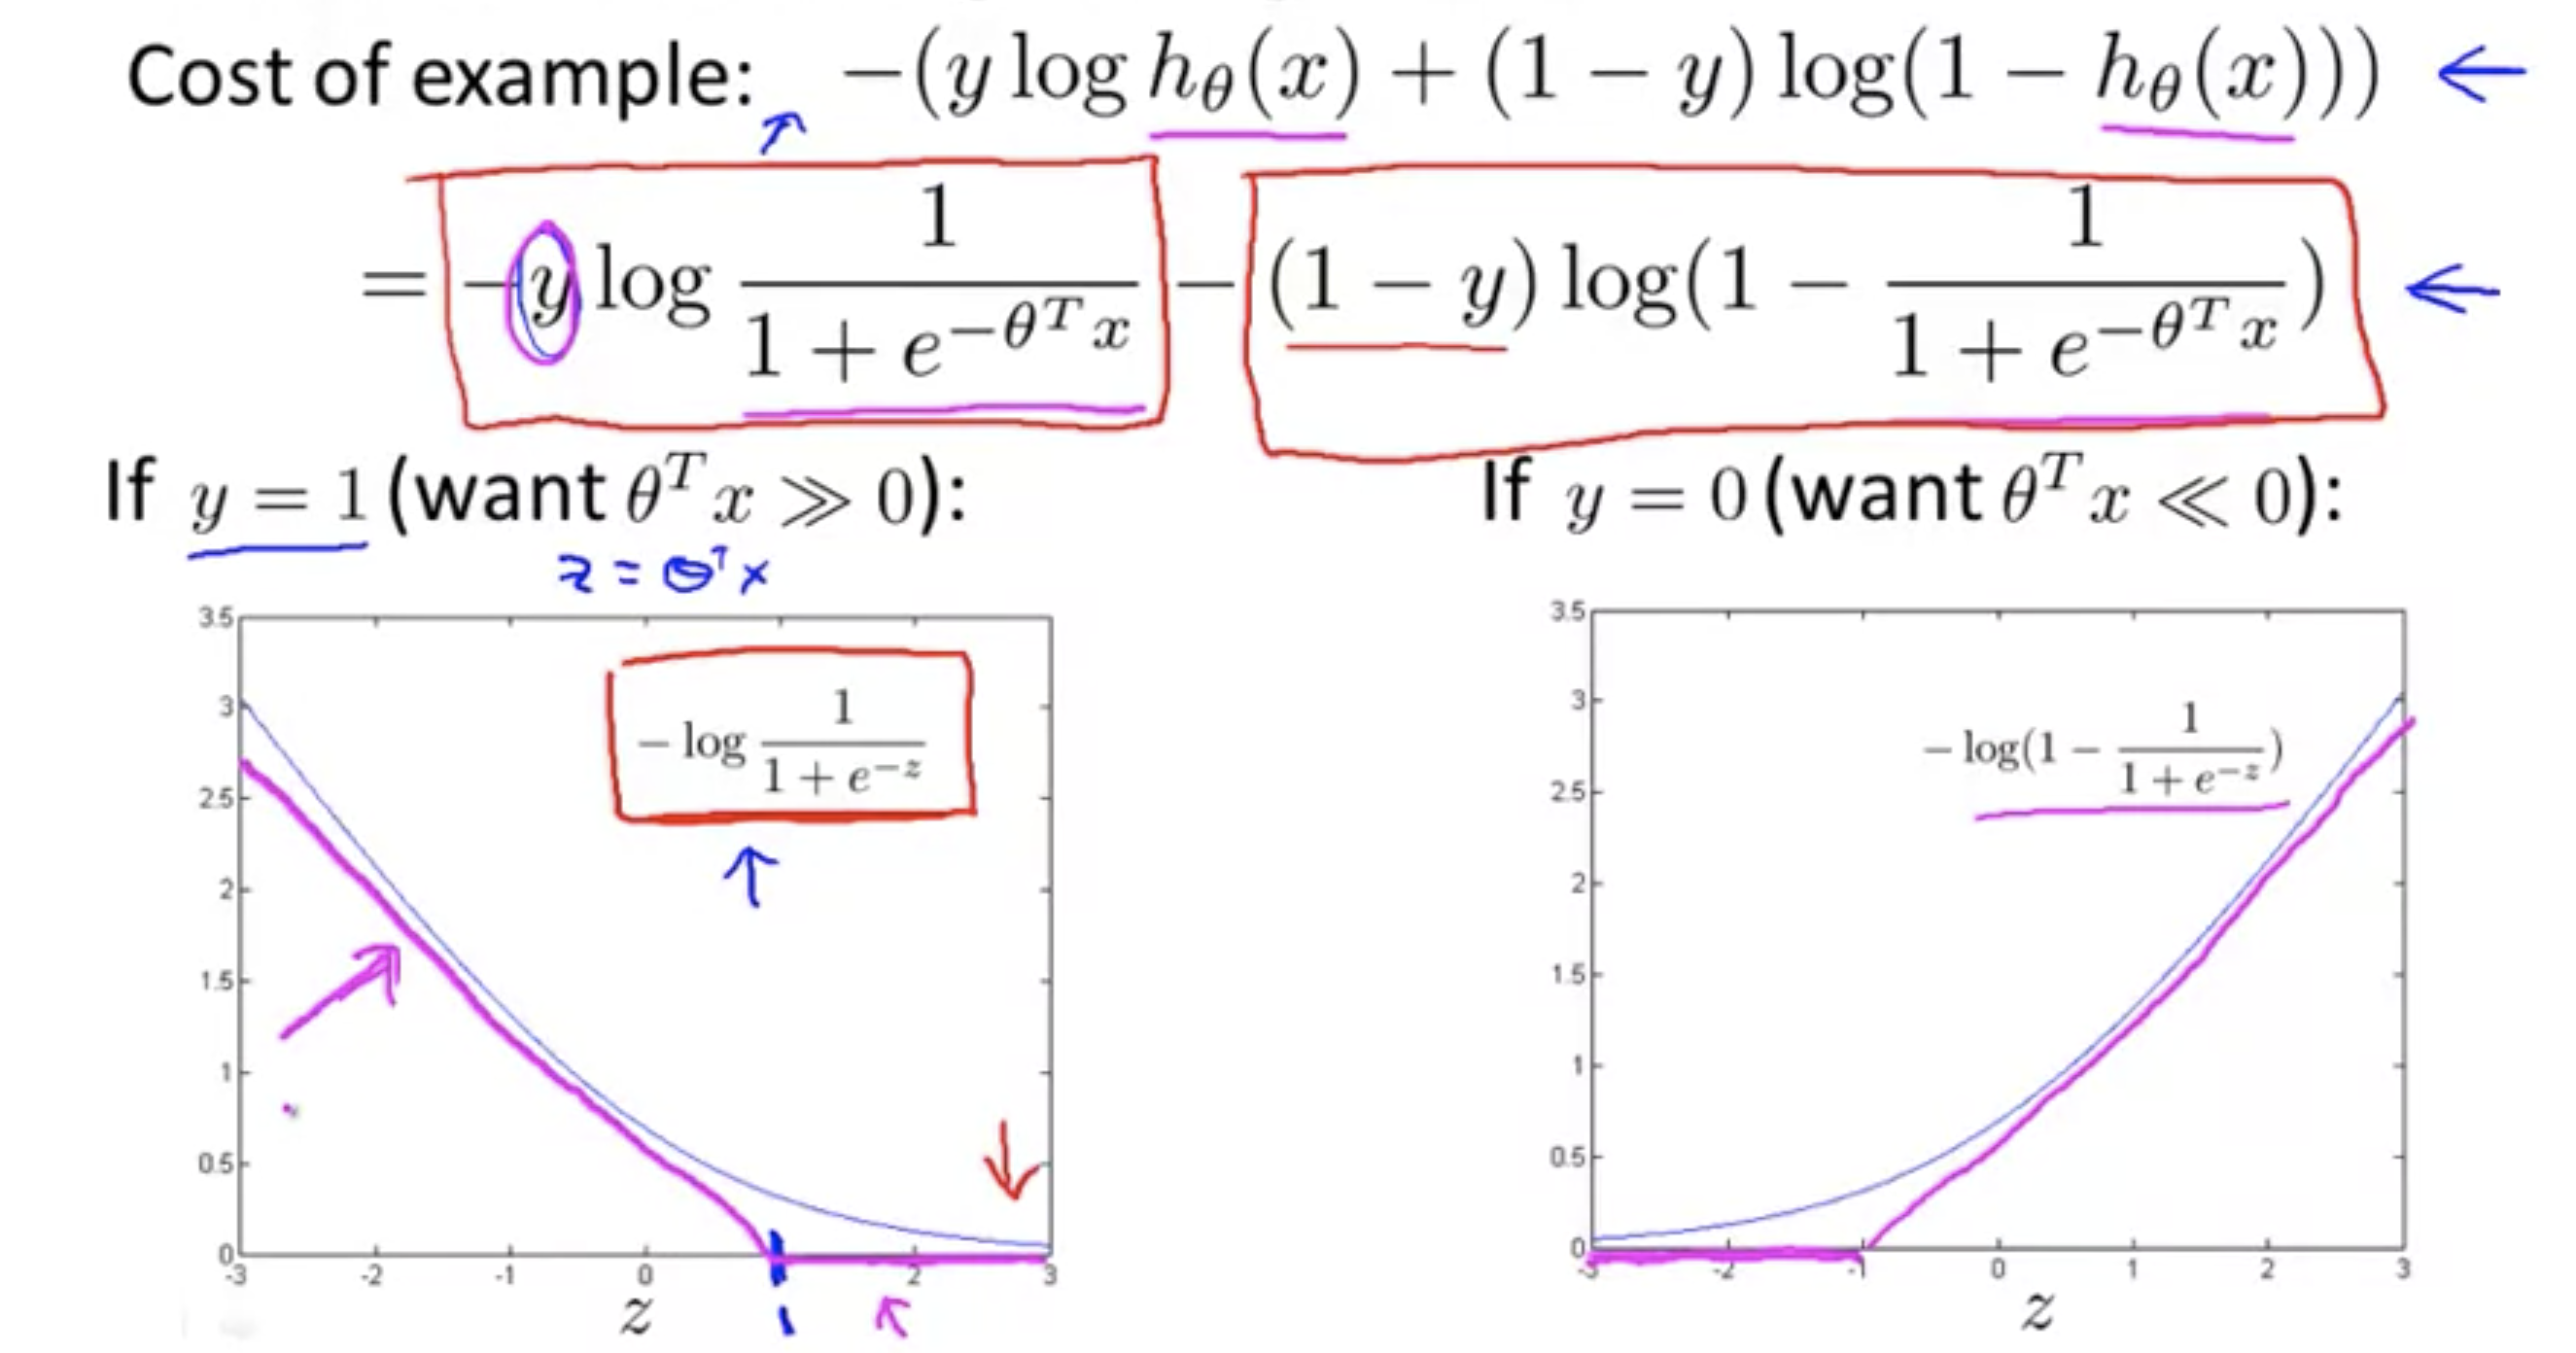
\includegraphics[width=0.7\textwidth]{fig/SVM}
	\caption{Logistic Cost example}
	\label{fig:svm}
\end{figure}

\pagebreak

Now, to fill the support vector machine, here's what we're going to do. We're gonna take this cross function, this on the left, and modify it a little bit. The new pass functions (drew in magenta) can be flat from here on out, and then we draw something that grows as a straight line, similar to logistic regression. But this is going to be a straight line at this portion. So the curve that I just drew in magenta, and the curve I just drew in purple and magenta, so it's pretty close approximation to the cross function used by logistic regression. Except it is now made up of two line segments, there's this flat portion on the right, and then there is this straight line portion on the left. \\

That's the new cost function we're going to use for when y is equal to one, and you can imagine it should do something pretty similar to logistic regression. But turns out, that this will give the support vector machine computational advantages and give us, later on, an easier optimization problem.\\

The other case is if y is equal to zero. In that case, if you look at the cost, then only the second term will apply because the first term goes away, right? If y is equal to zero, then you have a zero here, so you're left only with the second term of the expression. And for the support vector machine, once again, we're going to replace this blue line with something similar and at the same time we replace it with a new cost, this flat out here, this 0 out here. And that then grows as a straight line.\\

We're going to call this function on the left $ Cost_1(z) $ and this function of the right we're gonna call $ Cost_0(z) $. \\

The subscript just refers to the cost corresponding to when y is equal to 1, versus when y Is equal to zero.\\

So we have this SVM Cost function :

\begin{equation}
min_\theta  \hspace{0.2cm} C \sum_{i=1}^{m}\left( y^{(i)} Cost_1(\theta^T x) +(1- y^{(i)}) Cost_0(\theta^T x) \right) + \frac{1}{2}  \sum_{i=1}^{n} \theta_j^2
\end{equation}

\section{Large Margin Intuition}

Let's think about what it takes to make these cost functions small. If you have a positive example, (y is equal to 1), then $ Cost_1(z) $ is zero only when $ z \geq 1 $. So in other words, if you have a positive example, we really want theta transpose x to be greater than or equal to 1 and conversely if y is equal to zero, look this $ Cost_0(z) $ then it's only in this region where $ z \leq -1 $ we have the cost is zero as z is equals to zero.

\begin{figure}[h!]
	\centering
	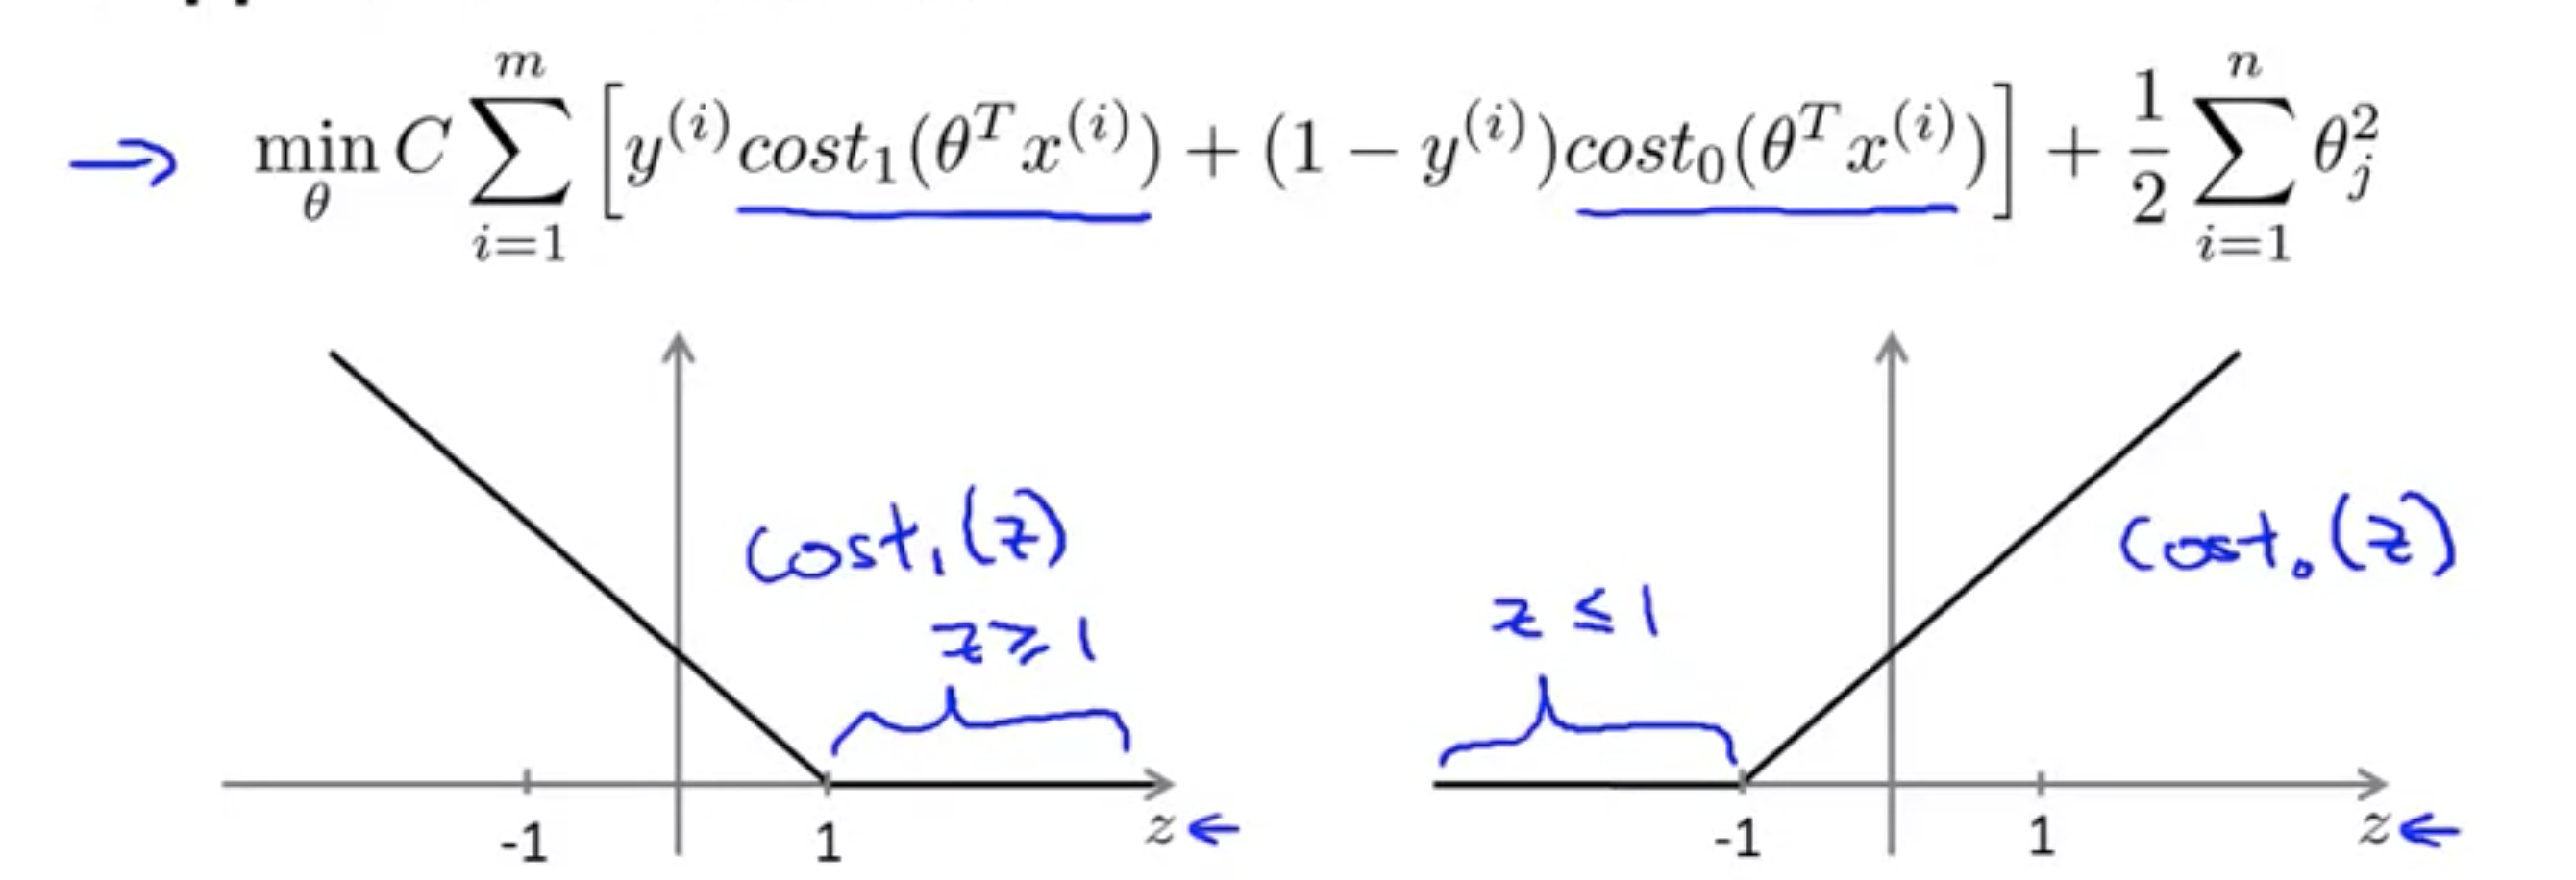
\includegraphics[width=0.7\textwidth]{fig/LMI_SVM_0}
	\caption{Large Marge Intuition}
	\label{fig:lmisvm0}
\end{figure}

In logistic regression, we take the output of the linear function and squash the value within the range of [0,1] using the sigmoid function. If the squashed value is greater than a threshold value(0.5) we assign it a label 1, else we assign it a label 0. In SVM, we take the output of the linear function and if that output is greater than 1, we identify it with one class and if the output is -1, we identify is with another class. Since the threshold values are changed to 1 and -1 in SVM, we obtain this reinforcement range of values([-1,1]) which acts as margin.\\

Using these support vectors, we maximize the margin of the classifier. Deleting the support vectors will change the position of the hyperplane (hypotheses). These are the points that help us build our SVM.

\begin{figure}[h!]
	\centering
	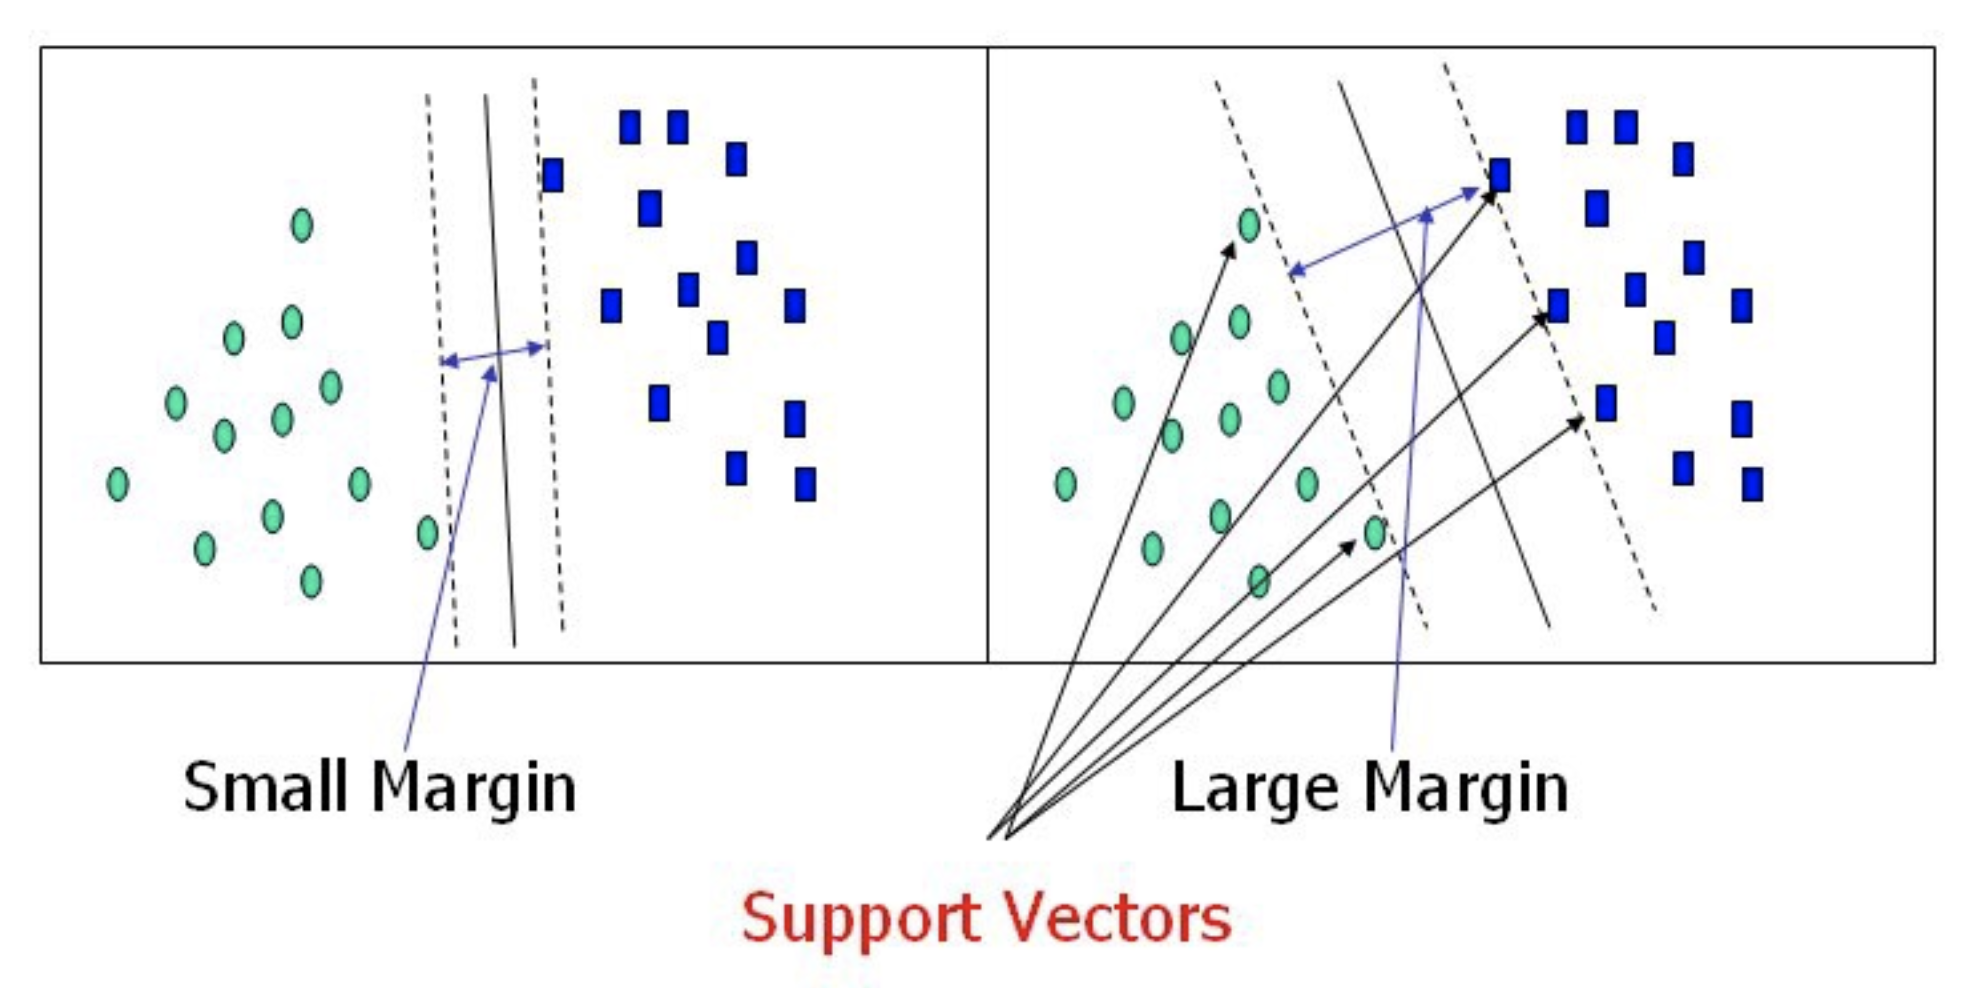
\includegraphics[width=0.7\textwidth]{fig/LMI_SVM}
	\caption{Large Marge Intuition}
	\label{fig:lmisvm}
\end{figure}